\chapter{Habitat of ice reservoirs}

AIRs cannot be built anywhere. They require sufficient water supply and weather conditions cold enough to
amass a seasonal stock of ice. This imposes several meteorological and topographical requirements for the chosen
construction location. The meteorological requirements can be used to identify favourable regions worldwide
whereas the topographical requirements can be used to pinpoint the construction site within the respective
region. Below we detail these requirements and propose methodologies for finding construction sites satisfying
them. 

\begin{figure}[t]
\centering
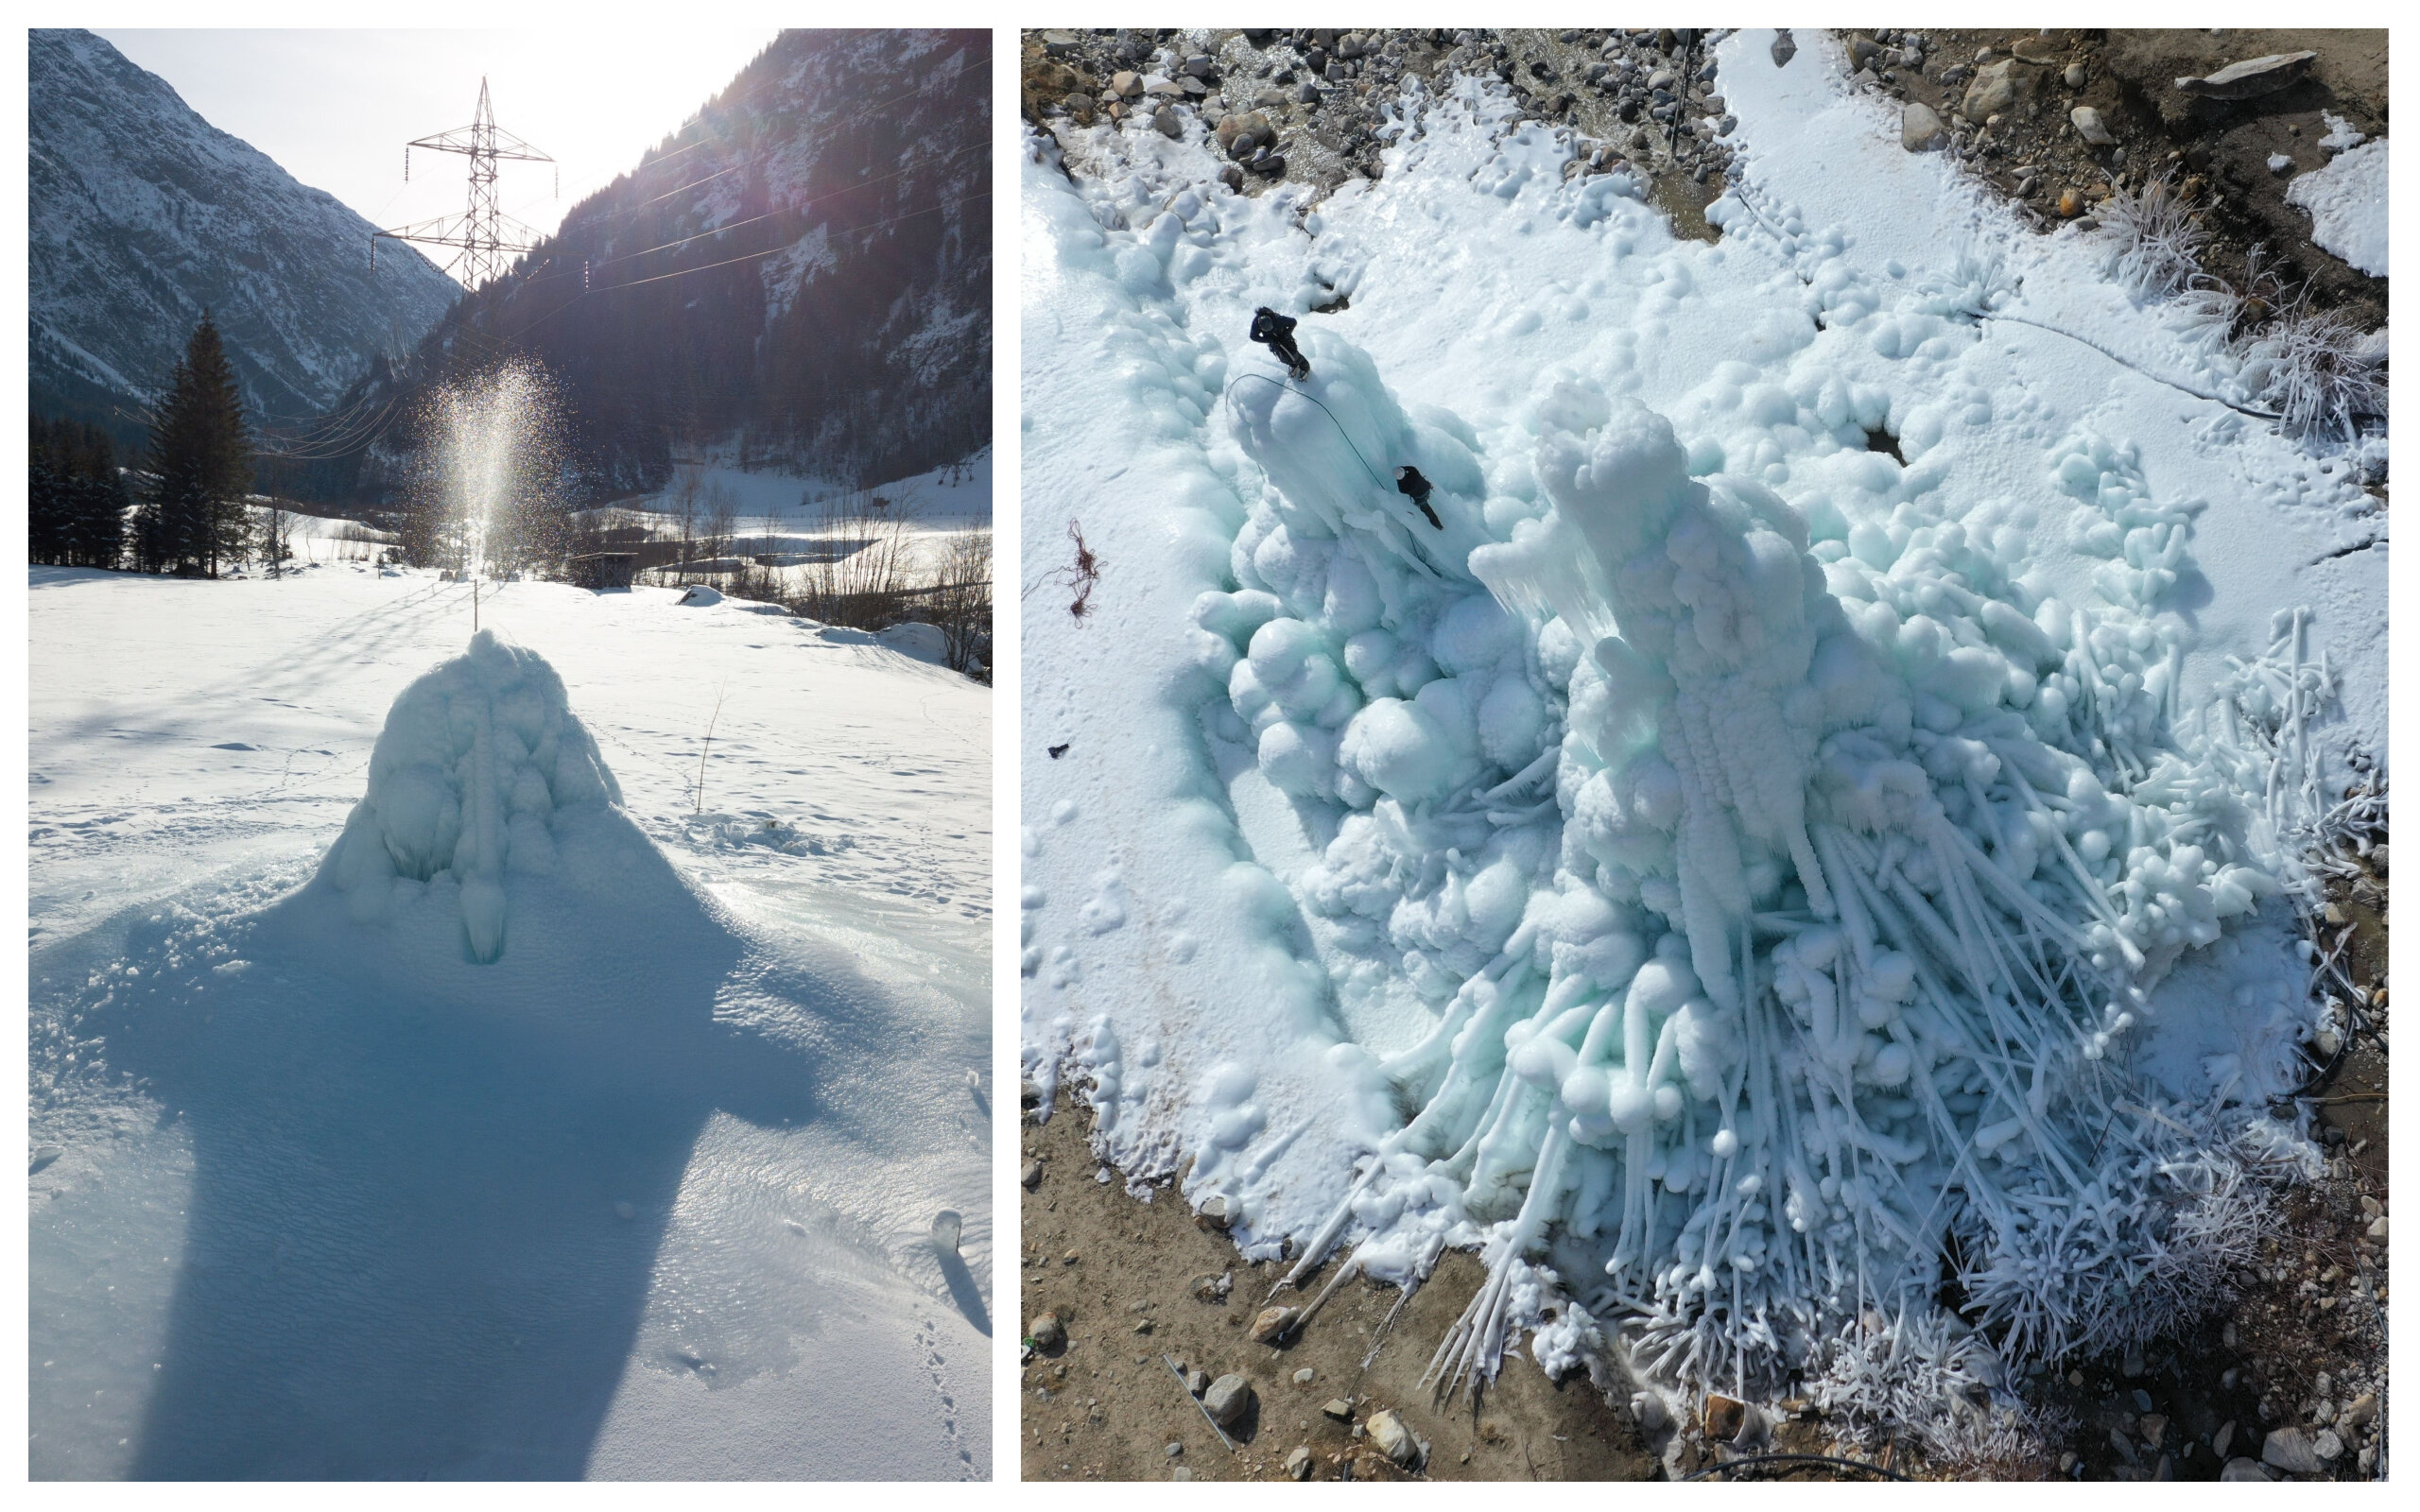
\includegraphics[width=12cm]{Figures/2AIRs.jpg}
\caption{AIRs show significant variation in volume evolution depending on the choice of construction location.}
\label{fig:2AIRs}
\end{figure}

\section{Requirements for AIR construction}

\begin{itemize}
  \item {\bf Water supply} : The water source of an AIR could be either a spring or a stream. Springs are the ideal
    water source since they are easy to transport via pipelines to the construction site due to their relatively
    warm temperatures. Other water sources have higher risks of pipeline freezing events. 

  \item {\bf Weather conditions} : AIRs prefer colder, drier and less-cloudy regions. Correspondingly,
    temperature, humidity and number of cloud-free days during the construction period can be used to rank
    different sites. 

  \item {\bf Topography} : AIRs prefer shadowed valleys. This is because these landforms have lower sunshine
    hours which is the major driver of the melting rate of all the AIRs studied in this thesis.

\end{itemize}


\subsection{Checklist to identify AIR construction regions}

Accordingly, we propose the following checklist to determine AIR site suitability. The values presented are
determined based on past construction experiences and can be used as guidelines to avoid construction attempts
in unfavourable sites.

\begin{enumerate}

  \item Minimum mean monthly temperature less than $0 \degree C$. 
  \item Water supply with mean discharge rate more than $2 l/min$. 
  \item Terrain slope between water source and site greater than 10 m every km. 

\end{enumerate}

\subsection{Metrics to rank sites within the same region }

Given a valley or a region satisfying the above requirements, further selection of sites around the particular
water supply can be performed using the criterions below: 

\begin{enumerate}
  \item Water source temperature is higher.
  \item Daylight hours are lower.
  \item Cloudy days are lower.
  \item Temperature is lower.
  \item Humidity is lower.
\end{enumerate}

Such villages are expected to produce AIRs that supply daily meltwater in the order of thousands of litres for 2
months. 

Different forms of AIRs show different sensitivities to each of these requirements. This is discussed in the
next chapter.
